% Created 2018-04-30 seg 16:35
% Intended LaTeX compiler: pdflatex
\documentclass[presentation]{beamer}
\usepackage[utf8]{inputenc}
\usepackage[T1]{fontenc}
\usepackage{graphicx}
\usepackage{grffile}
\usepackage{longtable}
\usepackage{wrapfig}
\usepackage{rotating}
\usepackage[normalem]{ulem}
\usepackage{amsmath}
\usepackage{textcomp}
\usepackage{amssymb}
\usepackage{capt-of}
\usepackage{hyperref}
\usepackage{graphicx, hyperref, udesc, url}
\usetheme{default}
\author{Rafael Castro - rafaelcgs10.github.io/coq}
\date{02/05/2018}
\title{Aula 1 - Introdução à introdução de Coq}
\hypersetup{
 pdfauthor={Rafael Castro - rafaelcgs10.github.io/coq},
 pdftitle={Aula 1 - Introdução à introdução de Coq},
 pdfkeywords={},
 pdfsubject={},
 pdfcreator={Emacs 25.3.1 (Org mode 9.1.11)}, 
 pdflang={Portuguese}}
\begin{document}

\maketitle

\section{Introducao}
\label{sec:org1ebf18b}

\begin{frame}[label={sec:org17ed56d}]{Provadores Automáticos}
\begin{itemize}
\item Entre com uma proposição, aperte um botão e veja a resposta.
\item Fazem todo o trabalho da prova. Humanos não são necessários.
\item São procedimentos de decisão.
\item Limitados a domínios específicos.
\item Fornecem um formalismo para especificar a proposição, mas não para a sua prova. Fornecem uma valoração caso falso.
\end{itemize}
\end{frame}
\begin{frame}[label={sec:org8a6c43a}]{Assistentes de Provas}
\begin{itemize}
\item São provadores semi-automáticos.
\item Uso com domínio menos restrito: podem falar sobre diversas lógicas, teorias e até mesmo programas.
\item Podem utilizar provadores automáticos, mas ainda necessitam do humano.
\item Fornecem um formalismo para representar a prova. \emph{Lembra} as regras da Dedução.
\end{itemize}
\end{frame}

\begin{frame}[label={sec:org97a41b7}]{Como Assistentes de provas assistem?}
\begin{itemize}
\item O núcleo de um assistente de provas é um verificador, que verifica a consistência lógica da prova.
\item A verficação humana de provas é demorada e sujeita a falhas: Último Teorema de Fermat.
\item Fornecem de maneira interativa de visualizar as informações sobre o estado atual da prova.
\item Ajudam a encontrar teoremas e lemas para o progresso da prova.
\item Permitem implementar métodos não-deterministas para auxiliar a prova.
\end{itemize}
Assistentes de provas permitem provar coisas que não seriam 
realizáveis somente com papel e caneta: Four Color Theorem
\begin{center}
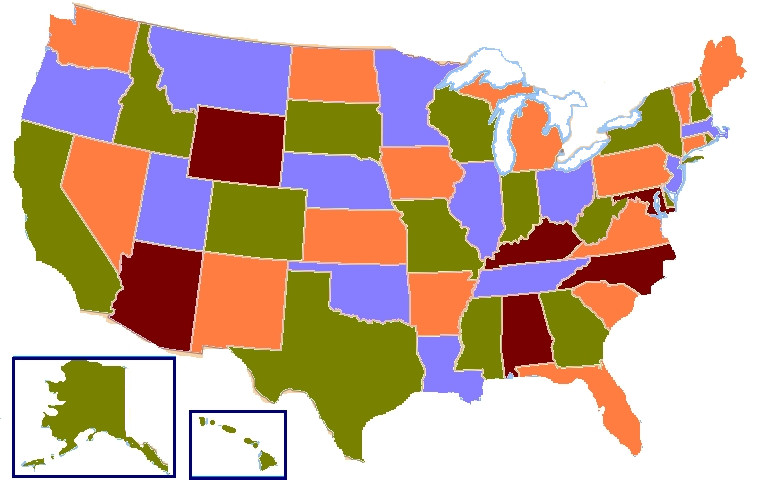
\includegraphics[width=60]{./four.jpeg}
\end{center}
\end{frame}

\begin{frame}[label={sec:org85d8006}]{Qual assistente utilizar?}
\begin{itemize}
\item Existem diversos assistentes, cada um baseado numa teoria matemática e com as suas peculiaridades:
Agda, Isabelle, HOL, Minlog, Coq\ldots{}
\item Iremos utilizar Coq! Mas por que?
\begin{enumerate}
\item É o que eu sei algo;
\item Existe desde 1984;
\item Há vários livros;
\item Suporte para ordem superior, tipos dependentes, automação e extração de código.
\end{enumerate}
\end{itemize}
\end{frame}

\begin{frame}[label={sec:orgf53f0f2}]{O que é Coq?}
\begin{itemize}
\item Coq é um assistentes de provas (dã) desenvolvido desde 1984 pelo French Institute for Research in Computer Science and Automation (INRIA).
\item Coq é fruto de sistemas de tipos: \alert{Higher order dependently typed polymorphic lambda calculus}, o nomeado Calculus of Constructions (CoC).
\item Inicialmente chamado de CoC, foi estendido em 1991 para suportar construções indutivas e o nome mudou para Coq. Referência a Thierry Coquand.
\item Coq tem quatro linguagens:
\begin{enumerate}
\item Gallina: linguagem de programação funcional total e com tipos dependentes.
\item Tatic: linguagem para criar provas com a ajuda do assistente/verificador.
\item Vernecular: linguagem de comandos. Enunciar teoremas, funções\ldots{}
\item LTac: criação de novas táticas e procedimentos de prova.
\end{enumerate}
\end{itemize}
\end{frame}

\begin{frame}[label={sec:orgf72259e}]{Programação certificada em Coq}
\begin{itemize}
\item Coq permite não só provar teoremas da matemática, mas também provar propriedades de programas.
\item Provar correturede de programas. \emph{Dijkstra screams in pleasure}
\item Programas verificados (ou provas) em Coq podem ser extraídos para outras linguagens como Haskell, OCaml e Scheme.
\end{itemize}
\end{frame}

\begin{frame}[label={sec:org1da307d}]{Como aprender Coq?}
Vamos utilizar o Volume 1 do Software Foundations 
\url{https://softwarefoundations.cis.upenn.edu/}
\begin{center}
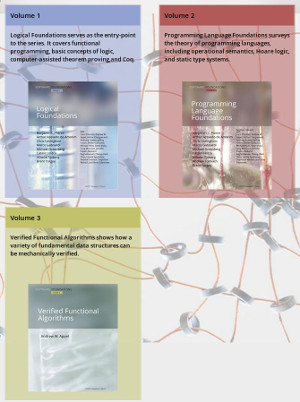
\includegraphics[width=100px]{./sf.jpeg}
\end{center}
\end{frame}

\begin{frame}[label={sec:org1508af0}]{Coq é confiável?}
No que eu preciso confiar quando vejo uma prova em Coq? 
\begin{itemize}
\item \alert{A teoria por trás de Coq}: Coq 8.0 é equivalente a Zermelo-Fraenkel set theory + inaccessible cardinals.
\item \alert{A implementação do núcleo do Coq}: A implementação representa a teoria por trás de Coq e é pequena para evitar o risco de erros.
\item \alert{O compilador de OCaml}: Utiliza somente bibliotecas básicas, então é improvável que um bug no compilador quebre a lógica de Coq sem quebrar todo os outros softwares feitos em OCaml.
\item \alert{Seu hardware}: Se o seu hardware falhar, pode ser possível provar o Falso (illuminati confirmed). Teste em outros computadores.
\item \alert{Seu sistema operacional}: idem hardware.
\item \alert{Seus axiomas}: Coq permite você adicionar novos axiomas, os quais precisam ser consistentes com a teoria de Coq.
\end{itemize}
\end{frame}

\section{Baby's First Steps}
\label{sec:orga9cdf13}

\begin{frame}[label={sec:org9922607}]{Como utilizar o assistente de provas?}
\begin{itemize}
\item CoqIDE = Bom lugar para começar sem perder o foco. Tem os recursos básicos.
\item Emacs + ProofGeneral + Company-coq = a maneira mais eficiente de usar Coq.
\end{itemize}
\end{frame}

\begin{frame}[fragile,label={sec:org5b1f76f}]{Baby's First Type}
 \begin{itemize}
\item Coq não tem um conjunto de dados básicos \emph{build-in}. Todos os tipos de Coq são definidos em Coq.
\item Tipos são definidos com \emph{Inductive}, seguido do identificador, o tipo desse tipo e a sua definição em \emph{| termo : tipo}.
\end{itemize}
\begin{verbatim}
Inductive day : Type :=
  | monday : day
  | tuesday : day
  | wednesday : day
  | thursday : day
  | friday : day
  | saturday : day
  | sunday : day.
\end{verbatim}
\end{frame}

\begin{frame}[fragile,label={sec:org955f9f3}]{Baby's First Proof}
 \begin{itemize}
\item Teoremas são enunciados com \emph{Theorem}, seguido do seu identificador e a sua proposição (tipo).
\item Provas são enunciadas com \emph{Proof} e finalizadas com \emph{Qed}.
\end{itemize}
\begin{verbatim}
Theorem fridayIsFriday : friday = friday.
Proof.
  reflexivity.
Qed.
\end{verbatim}
\end{frame}
\end{document}